\documentclass[presentation]{beamer}
\usepackage{hyperref}
\usepackage{color}
\usepackage{listings}
\usepackage{multicol}

\usepackage{tikz}
\usetikzlibrary{graphs}
\usetikzlibrary{quotes}

\usetheme{Madrid}

\author{Hebi Li, James Nhan}

\title{Automated Project Rater}
\begin{document}
\maketitle


\begin{frame}{Outline}
\tableofcontents
\end{frame}


\section{Problem Definition}
\begin{frame}{Problem Definition}
  Given a project, predict the quality of it using simple and easy to
  get file level features.
\end{frame}


\begin{frame}{Motivation}
\begin{itemize}
\item Open Source Projects are of different qualities
\item Hard to tell the quality without a proper rating accumulated by
  user (like GitHub stars)
\item Useful for company searching for tools
\item Useful for learners and contributors to select good projects
\end{itemize}
\end{frame}

\begin{frame}{Challenges}
  \begin{itemize}
  \item No data sets available
  \item Complex features are hard to get
    \begin{itemize}
    \item Control flow features such as program dependence, call graph,
      def use information, symbol table are expensive to get
    \item Data stored on server requires using API (e.g. GitHub API)
    \item They typically have access limit (e.g. GitHub API allows only
      \textbf{30 requests per minute} for authenticated user)
    \end{itemize}
  \item Simple features might not be able to express the rating
  \end{itemize}
\end{frame}

\section{Related Work \& Contribution}
\begin{frame}{Related Work}
  Related Work
  \begin{itemize}
  \item No previous work has been done to rate project quality
  \item No such data set is public available
  \item Some research in MSR is related. E.g. OpenHub
    \footnote{OpenHub: A Scalable Architecture for the Analysis of
      Software Quality Attributes, MSR 2014, Farah, Gabriel et al.},
    Documentation mining \footnote{On Mining Crowd-based Speech
      Documentation, MSR '16, Moslehi, Parisa et al.}. See the related
    work section in our paper.
  \end{itemize}

  Our contribution
  \begin{itemize}
  \item Publicly available data set for 10000 projects with
    15 features each with GitHub star number as ground truth.
  \item Analyze the data set and features using linear regression, SVM
    with linear and non-linear kernels, decision tree approaches
  \end{itemize}
\end{frame}


\section{Workflow}
\begin{frame}{Workflow}
% Github Search API -> 
% -> downloader -> feature extractor -> analyzer -> predict model

  \centering
  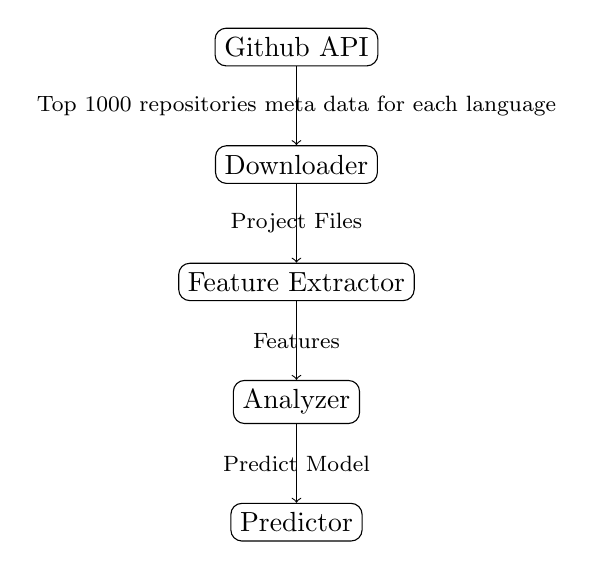
\begin{tikzpicture}
    \graph[grow down sep=1cm, nodes={draw, rounded corners},
    edge quotes={font=\footnotesize}] {
    githubapi/"Github API" -> ["Top 1000 repositories meta data for each language"]
    downloader/"Downloader" -> ["Project Files"]
    extractor/"Feature Extractor" -> ["Features"]
    analyzer/"Analyzer" -> ["Predict Model"]
    predictor/"Predictor"
  };

  % \graph[grow right sep=2cm] {
  %   github api -> b -> c;
  % };
  
  % \node (githubapi) at (0,0) {Github API};
  % \node (downloader) at (4,0) {Downloader};
  % \node (extractor) at (4,0) {Feature Extractor};
  % \node (analyzer) at (6,0) {Analyzer};

  % \draw[->] (githubapi) -- (downloader) -- (extractor) -- (analyzer);
\end{tikzpicture}

\end{frame}


\section{Data Collection}
\begin{frame}{Ground Truth}
  We use GitHub star number as ground truth.
\end{frame}

\begin{frame}{Feature}
  \begin{multicols}{2}
    A list of features
    \begin{itemize}
    \item has download?
    \item has issue?
    \item has wiki?
    \item has page?
    \item open issue
    \item size
    \item test file
    \item doc file
    \item src file
    \item loc
    \item comment
    \item file depth
    \item file count
    \item dir branching factor
    \item dir count
    \item fork count
    \end{itemize}
  \end{multicols}
\end{frame}


\begin{frame}{Data Collection}
\begin{enumerate}
\item Use GitHub search APIs to query top 1000 projects by star number
  \begin{itemize}
  \item Languages used: C, Java, JavaScript, shell,
    Python, Ruby, PHP
  \item GitHub search API can at most return 1000 for a search
  \item We are interested in the top rated projects.
  \item 1000 projects roughly containing projects rating from 300
    stars to 10,000-30,000 stars
  \item Different languages can
    \begin{itemize}
    \item Give us overall result regardless of language
    \item Show which language works best
    \item Compare results across languages
    \end{itemize}
  \end{itemize}
\item Download projects
\item Extract features
\end{enumerate}
\end{frame}

\begin{frame}{Data Collection Continued}
\begin{enumerate}
\item use GitHub search APIs to query top 1000 projects by star number
\item Download projects
  \begin{itemize}
  \item We analyze the features using scripts offline, to avoid the
    query rate limit posed by GitHub
  \end{itemize}
\item Extract features
  \begin{itemize}
  \item Features are stored into SQLite database for query and update
  \item Final features and response (ground truth star number) are
    written into csv file for analyze
  \end{itemize}
\end{enumerate}
\end{frame}

\section{Model Training}
\begin{frame}{Analysis Algorithm}
\begin{itemize}
% \item linear model
\item Support Vector Machine with kernels:
  \begin{itemize}
  \item Linear
  \item Polynomial
  \item Radial Basis
  \item Sigmoid
  \end{itemize}
% \item Decision Tree
\end{itemize}
\end{frame}

\begin{frame}{Analysis Algorithm Continued}
We didn't tune the parameters because of less of precise knowledge
about how to tune them. Model selection turns out to be a issue for
the data set that is new and not familiar.
\end{frame}


\section{Result \& Conclusion}
\begin{frame}{Results}
  
  \begin{figure}[ht]
    \centering
    \includegraphics[height=0.8\textheight]{star-hist.png}
    % \caption{Data set visualization}
  \end{figure}

\end{frame}


\begin{frame}{Model Prediction Visualization}
  \begin{figure}[ht]
    \scriptsize
    \centering
    \includegraphics[width=0.3\textwidth]{images/wholepng/whole-linear.png}
    \includegraphics[width=0.3\textwidth]{images/wholepng/whole-polynomial.png}\\
    \includegraphics[width=0.3\textwidth]{images/wholepng/whole-radial.png}
    \includegraphics[width=0.3\textwidth]{images/wholepng/whole-sigmoid.png} 
    \caption{Linear, Polynomial, Radial Basis, Sigmoid kernels}
  \end{figure}
\end{frame}

\begin{frame}{Model Prediction Visualization}
  \begin{figure}[ht]
    \scriptsize
    \centering
    \includegraphics[width=0.3\textwidth]{images/langpng/c-linear.png}
    \includegraphics[width=0.3\textwidth]{images/langpng/c-radial.png}\\
    \includegraphics[width=0.3\textwidth]{images/langpng/javascript-linear.png}
    \includegraphics[width=0.3\textwidth]{images/langpng/javascript-radial.png}\\
    \caption{Linear(Left) and Polynomial(Right), for C(top) and JavaScript(Bottom)}
  \end{figure}
\end{frame}

\begin{frame}{Model Prediction Visualization}
  \begin{figure}[ht]
    \scriptsize
    \centering
    \includegraphics[width=0.3\textwidth]{images/langpng/python-linear.png}
    \includegraphics[width=0.3\textwidth]{images/langpng/python-radial.png}\\
    \includegraphics[width=0.3\textwidth]{images/langpng/ruby-linear.png}
    \includegraphics[width=0.3\textwidth]{images/langpng/ruby-radial.png}\\
    \caption{Linear(Left) and Polynomial(Right), for Python(top) and Ruby(Bottom)}
  \end{figure}
\end{frame}

\begin{frame}{Results Continued}
  Support Vector Machine with Variety of Models
  \begin{table}
    \centering
    \begin{tabular}{r|r}
      Category & Accuracy\\
      \hline
      2 & 0.83\\
      3 & 0.71\\
      4 & 0.61\\
      5 & 0.54\\
      6 & 0.47\\
      7 & 0.42\\
      8 & 0.38\\
      9 & 0.35\\
      10 & 0.32\\
    \end{tabular}
    \caption{Discretization v.s. Accuracy}
  \end{table}
\end{frame}

\begin{frame}{Results Continued}
  \begin{table}
    \centering
    \scriptsize
    \begin{tabular}{r|r|r|r|r|r|r|r}
      Category & c.csv & php.csv & java.csv & javascript.csv & shell.csv & ruby.csv & python.csv\\
      \hline
      2 & 0.92 & 0.93 & 0.84 & 0.56 & 0.95 & 0.88 & 0.83\\
      3 & 0.85 & 0.87 & 0.7 & 0.39 & 0.92 & 0.78 & 0.74\\
      4 & 0.79 & 0.82 & 0.61 & 0.31 & 0.87 & 0.69 & 0.63\\
      5 & 0.76 & 0.76 & 0.52 & 0.22 & 0.82 & 0.63 & 0.56\\
      6 & 0.72 & 0.71 & 0.47 & 0.17 & 0.8 & 0.58 & 0.51\\
      7 & 0.67 & 0.67 & 0.42 & 0.15 & 0.77 & 0.53 & 0.46\\
      8 & 0.63 & 0.63 & 0.36 & 0.15 & 0.74 & 0.49 & 0.42\\
      9 & 0.6 & 0.59 & 0.33 & 0.11 & 0.71 & 0.46 & 0.39\\
      10 & 0.57 & 0.57 & 0.3 & 0.1 & 0.69 & 0.44 & 0.35\\
    \end{tabular}
    \caption{Compare across different languages}
  \end{table}
  
\end{frame}

\begin{frame}{Results Continued}
  \begin{table}
    \centering
    \begin{tabular}{r|r|r|r|r}
      Category & Linear & Polynomial & Radial & Sigmoid\\
      \hline
      2 & 0.82 & 0.82 & 0.83 & 0.8\\
      3 & 0.71 & 0.69 & 0.71 & 0.67\\
      4 & 0.61 & 0.58 & 0.61 & 0.58\\
      5 & 0.54 & 0.49 & 0.54 & 0.5\\
      6 & 0.47 & 0.43 & 0.47 & 0.45\\
      7 & 0.42 & 0.36 & 0.43 & 0.4\\
      8 & 0.38 & 0.33 & 0.38 & 0.36\\
      9 & 0.35 & 0.29 & 0.35 & 0.33\\
      10 & 0.32 & 0.26 & 0.32 & 0.29\\
    \end{tabular}
    \caption{Different Kernels}
  \end{table}

\end{frame}

\begin{frame}{Conclusions \& Future Work}
  Our research shows that,
  \begin{itemize}
  \item The features we use can be used to predict the quality.
  \item Different kernels, without tuning of parameters, do not have
    much different performance.
  \end{itemize}

  Future Work
  \begin{itemize}
  \item More advanced features
  \item Resolve bias of data (e.g. more projects with lower stars)
  \item Integrate with other research
  \end{itemize}
\end{frame}

\end{document}
